
\documentclass[]{article}
\voffset=-1.2cm
\oddsidemargin=0.0cm
\textwidth = 470pt
\usepackage[utf8]{inputenc}
\usepackage[english]{babel}
\usepackage{framed}
\usepackage{graphicx}
\usepackage{enumerate}% http://ctan.org/pkg/enumerate
\usepackage{multicol}
\usepackage{amsmath}
\usepackage{amssymb}
%=========================================================================================== %

\begin{document}

\subsection*{Question 1:  Sequences and Series}

\begin{enumerate}
	\item[(i)] Find the sum of the first 10 numbers of this arithmetic series: $1 + 11 + 21 + 31 + \ldots$
	
	\item[(ii)] 
	The second term $u_2$ of a geometric sequence is 21.
	
	The third term $u_3$ is -84.
	\begin{itemize}
		\item Find the common ratio 
		\item Find the first and fourth term
	\end{itemize}
	%- Page 16
	
	\item[(iii)] Three consecutive terms of an arithmetic series are \[4x - 1, 2x +11, 3x + 41. \]
	Find the value of x.
	%answer is 460
	
	\item[(iv)] Find the sum of the following geometric series: 
	\[3 + 6 + 12 + 24 + \ldots + 1536\]
	
	%----------------------------------%
	\item[(v)] 
	
	In an arithmetic sequence, three consecutive terms have a sum of - 9 and a product of 48.
	Find the common difference $d$ for these terms.
	\\
	\textit{\textit{Hint : Write terms as $x-d,x,x+d$}}
	%----------------------------------%
	\item[(vi)]
	The first three terms of an arithmetic sequence are 6,-9 and x.
	The first three terms of a geometric sequence are 6, x, y.
	Find the value of $x$ and the value of $y$.
	
	%---------------------------------%
	\item[(vii)]
	Find the sum to infinity of the geometric series
	
	\[ 1 + \bigg(\frac{2}{3}\bigg) + \bigg(\frac{2}{3}\bigg)^2 + \bigg(\frac{2}{3}\bigg)^2 + \ldots \]
	%-----------------------------------%
	\item[(viii)]
	The first three terms of a geometric series are
	
	\[ x-2 , 2x+3, 7x \]
	
	Find both of the possible values of $x$
	
	%- Page 27
	
	%----------------------------------%
	\item[(ix)]
	The $n-$th term of an arithmetic is $3n+2$
	
	Find $S_n$ the sum of the first $n$ terms, in terms of $n$
\end{enumerate}
\newpage


\subsection*{Question 2 : Convergence of a Sequence}

\begin{framed}
	A sequence $u_n$
	is said to converge to a limit $L$ where $L \neq \infty$ if
	\[ \lim_{n \to \infty } u_n = L \]
	
	
	
	
	If a sequence does not converge then it is said to be divergent. \end{framed}
%
%\begin{itemize}
%\item  Unless explicity told to use the Ratio test, you may use this approach.
%\end{itemize}
Test the following sequences for convergence. see page 14 of notes for more details.
\begin{multicols}{2}
	\begin{itemize}
		\item[(i)] \[u_n = \frac{2n-1}{4n+3}\]
		
		\item[(ii)] \[u_n = \frac{n+5}{3n+4}\]
		
		\item[(iii)] \[u_n = \frac{n+4}{2n^3 + n +3}\]
		
		\item[(iv)] \[u_n = \frac{n^2 +5n }{n^2 + 2n -1}\]
		
		\item[(v)] \[u_n = \frac{2n^3+1}{2n^3 +3n +4 } \]
		
		\item[(vi)]\[u_n =  \frac{2n^4+1}{n^3 +2n^2 -1 } \]
		
	\end{itemize}	
\end{multicols}
%====================================%
\subsection*{Question 15 : The Ratio test}


	\begin{framed}
		\noindent For a series with general term $u_n$, if
		
		\[ \lim_{n \to \infty } \left| \frac{u_{n+1}}{u_n} \right| = r\]
		then
		
		\begin{itemize}
			\item the series converges (absolutely) if $r<1$
			\item the series diverges if $r>1$ (or if r is infinity)
			\item the series could do either if $r=1$, so the test is not conclusive.
		\end{itemize}
	\end{framed}
\noindent \textit{This formula will be given in the back of the exam paper. However the indications on how to interpret $r$ will not be given.}
	\begin{framed}
		\subsubsection*{Example}
		Suppose that the following term is the general term for a series. Test this series for convergence
		
		\[u_n=\frac{n!n!}{(2n)!}\]
		then
		
		\[\frac{u_{n+1}}{u_n}=\frac{(n+1)^2}{(2n+1)(2n+2)}=\frac{n+1}{4n+2} \]
		\[ \to \frac{1}{4}\]
		so this series converges.
	\end{framed}
	
	
	
	
	\noindent Use the Ratio Test to test the following series for convergence
	\begin{multicols}{2}
		\begin{itemize}
			\item[(i)] 
			\[\sum^{\infty}_{n=1} \frac{x^{n+1}}{4^n} \]
			\item[(i)] 
			\[\sum^{\infty}_{n=1} \frac{4^n}{(n+1)!} \]
			
			\item[(iii)] \[\sum^{\infty}_{n=1} \frac{5^n }{n!} \]
			
			
			\item[(iv)] \[\sum^{\infty}_{n=1} \frac{n+1}{2^n} \]
			
		\end{itemize}
	\end{multicols}
	
	\begin{itemize}
		\item[(v)] Use the Ratio test to find the values for $x$ for which the series  is convergent
		\[\sum^{\infty}_{n=1} \frac{x^{n} }{n+2} \]
		
	\end{itemize}
	

\subsection*{Question 24 : Calculations for the Ratio Test}

For each of the following terms, given as $u_n$, state $u_{n+1}$ and hence calculate a simplified expression for $r$, where 
{
	\Large
	\[ r = \frac{u_{n+1}}{u_n}\]
}
{
	\Large
	\begin{multicols}{2}
		\begin{itemize}
			\item[(i)]  $u_n = \displaystyle{n^2}$\smallskip
			\item[(ii)] $u_n = \displaystyle{2^n}$ \smallskip
			\item[(iii)] $u_n = \displaystyle{\frac{2^n}{n^2}}$ \smallskip
			\item[(iv)] $u_n = (2n)!$
			\item[(v)] $u_n = \displaystyle{\frac{2^n}{n!}}$ \smallskip
			\item[(vi)] $u_n = \displaystyle{\frac{2^n \times n}{n!}}$\smallskip
			\item[(vii)] $u_n = n! \times n!$
			\item[(viii)] $u_n = \displaystyle{\frac{2^{n+1} \times n^2}{ 4^n \times n!}}$
			
		\end{itemize}
	\end{multicols}
	\smallskip
}
%================================================================== %


\subsection*{Question 16 : Evaluation of telescoping series}

Find the sum of the following telescoping series
\begin{multicols}{2}
	\begin{itemize}
		\item[(i)]
		\[  \sum^{\infty}_{n=1}   \frac{3}{(3n+1)(3n+4)}  \]
		
		\item[(ii)]
		\[  \sum^{\infty}_{n=1}   \frac{4}{(2n+1)(2n+3)}  \]
		
		\item[(iii)]
		\[  \sum^{\infty}_{n=1}   \frac{5}{(5n+1)(5n+6)}  \]
		
		\item[(iv)]
		\[  \sum^{\infty}_{n=1}  \frac{6}{(6n+1)(6n+7)}  \]
		.
	\end{itemize}
\end{multicols}

%=========================================================== %
\bigskip

\subsection*{Question 17 : Evaluation of Telescoping Series}
Answer the following questions
\begin{itemize}
	% % Revise Cross Multiplication
	\item[(i)] Show that, where $r \neq \pm 1$.
	\[ \frac{2}{r^2-1} =  \frac{1}{r-1} - \frac{1}{r+1} \]
	% \item[(ii)] Hence, find the following summation
	
	% \[  \sum^{n}_{r=2} \frac{2}{r^2+1} \]
	\item[(ii)] Hence, evaluate the following summation
	\[  \sum^{n}_{r=2} \frac{2}{r^2-1} \]
	\item[(iii)] Hence, evaluate the following summation
	\[  \sum^{\infty}_{r=2} \frac{2}{r^2-1} \]
\end{itemize}


\bigskip

\subsection*{Question 18 : Evaluation of terms in a Maclaurin Series}
\large
\begin{itemize}
	\item[(i)] Evaluate the following Macluarin Series for $n=\{1,2,3\}$.
\end{itemize}
\begin{figure}[h!]
	\centering
	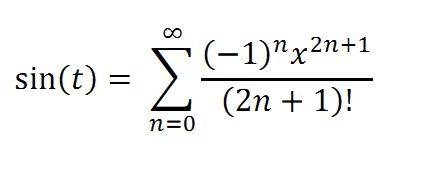
\includegraphics[width=0.30\linewidth]{macl3}
	%	\caption{}
	\label{fig:macl3}
\end{figure}

%========================================================================= %
\newpage

